\documentclass[1p]{elsarticle_modified}
%\bibliographystyle{elsarticle-num}

%\usepackage[colorlinks]{hyperref}
%\usepackage{abbrmath_seonhwa} %\Abb, \Ascr, \Acal ,\Abf, \Afrak
\usepackage{amsfonts}
\usepackage{amssymb}
\usepackage{amsmath}
\usepackage{amsthm}
\usepackage{scalefnt}
\usepackage{amsbsy}
\usepackage{kotex}
\usepackage{caption}
\usepackage{subfig}
\usepackage{color}
\usepackage{graphicx}
\usepackage{xcolor} %% white, black, red, green, blue, cyan, magenta, yellow
\usepackage{float}
\usepackage{setspace}
\usepackage{hyperref}

\usepackage{tikz}
\usetikzlibrary{arrows}

\usepackage{multirow}
\usepackage{array} % fixed length table
\usepackage{hhline}

%%%%%%%%%%%%%%%%%%%%%
\makeatletter
\renewcommand*\env@matrix[1][\arraystretch]{%
	\edef\arraystretch{#1}%
	\hskip -\arraycolsep
	\let\@ifnextchar\new@ifnextchar
	\array{*\c@MaxMatrixCols c}}
\makeatother %https://tex.stackexchange.com/questions/14071/how-can-i-increase-the-line-spacing-in-a-matrix
%%%%%%%%%%%%%%%

\usepackage[normalem]{ulem}

\newcommand{\msout}[1]{\ifmmode\text{\sout{\ensuremath{#1}}}\else\sout{#1}\fi}
%SOURCE: \msout is \stkout macro in https://tex.stackexchange.com/questions/20609/strikeout-in-math-mode

\newcommand{\cancel}[1]{
	\ifmmode
	{\color{red}\msout{#1}}
	\else
	{\color{red}\sout{#1}}
	\fi
}

\newcommand{\add}[1]{
	{\color{blue}\uwave{#1}}
}

\newcommand{\replace}[2]{
	\ifmmode
	{\color{red}\msout{#1}}{\color{blue}\uwave{#2}}
	\else
	{\color{red}\sout{#1}}{\color{blue}\uwave{#2}}
	\fi
}

\newcommand{\Sol}{\mathcal{S}} %segment
\newcommand{\D}{D} %diagram
\newcommand{\A}{\mathcal{A}} %arc


%%%%%%%%%%%%%%%%%%%%%%%%%%%%%5 test

\def\sl{\operatorname{\textup{SL}}(2,\Cbb)}
\def\psl{\operatorname{\textup{PSL}}(2,\Cbb)}
\def\quan{\mkern 1mu \triangleright \mkern 1mu}

\theoremstyle{definition}
\newtheorem{thm}{Theorem}[section]
\newtheorem{prop}[thm]{Proposition}
\newtheorem{lem}[thm]{Lemma}
\newtheorem{ques}[thm]{Question}
\newtheorem{cor}[thm]{Corollary}
\newtheorem{defn}[thm]{Definition}
\newtheorem{exam}[thm]{Example}
\newtheorem{rmk}[thm]{Remark}
\newtheorem{alg}[thm]{Algorithm}

\newcommand{\I}{\sqrt{-1}}
\begin{document}

%\begin{frontmatter}
%
%\title{Boundary parabolic representations of knots up to 8 crossings}
%
%%% Group authors per affiliation:
%\author{Yunhi Cho} 
%\address{Department of Mathematics, University of Seoul, Seoul, Korea}
%\ead{yhcho@uos.ac.kr}
%
%
%\author{Seonhwa Kim} %\fnref{s_kim}}
%\address{Center for Geometry and Physics, Institute for Basic Science, Pohang, 37673, Korea}
%\ead{ryeona17@ibs.re.kr}
%
%\author{Hyuk Kim}
%\address{Department of Mathematical Sciences, Seoul National University, Seoul 08826, Korea}
%\ead{hyukkim@snu.ac.kr}
%
%\author{Seokbeom Yoon}
%\address{Department of Mathematical Sciences, Seoul National University, Seoul, 08826,  Korea}
%\ead{sbyoon15@snu.ac.kr}
%
%\begin{abstract}
%We find all boundary parabolic representation of knots up to 8 crossings.
%
%\end{abstract}
%\begin{keyword}
%    \MSC[2010] 57M25 
%\end{keyword}
%
%\end{frontmatter}

%\linenumbers
%\tableofcontents
%
\newcommand\colored[1]{\textcolor{white}{\rule[-0.35ex]{0.8em}{1.4ex}}\kern-0.8em\color{red} #1}%
%\newcommand\colored[1]{\textcolor{white}{ #1}\kern-2.17ex	\textcolor{white}{ #1}\kern-1.81ex	\textcolor{white}{ #1}\kern-2.15ex\color{red}#1	}

{\Large $\underline{10_{58}~(K10a_{20})}$}

\setlength{\tabcolsep}{10pt}
\renewcommand{\arraystretch}{1.6}
\vspace{1cm}\begin{tabular}{m{100pt}>{\centering\arraybackslash}m{274pt}}
\multirow{5}{120pt}{
	\centering
	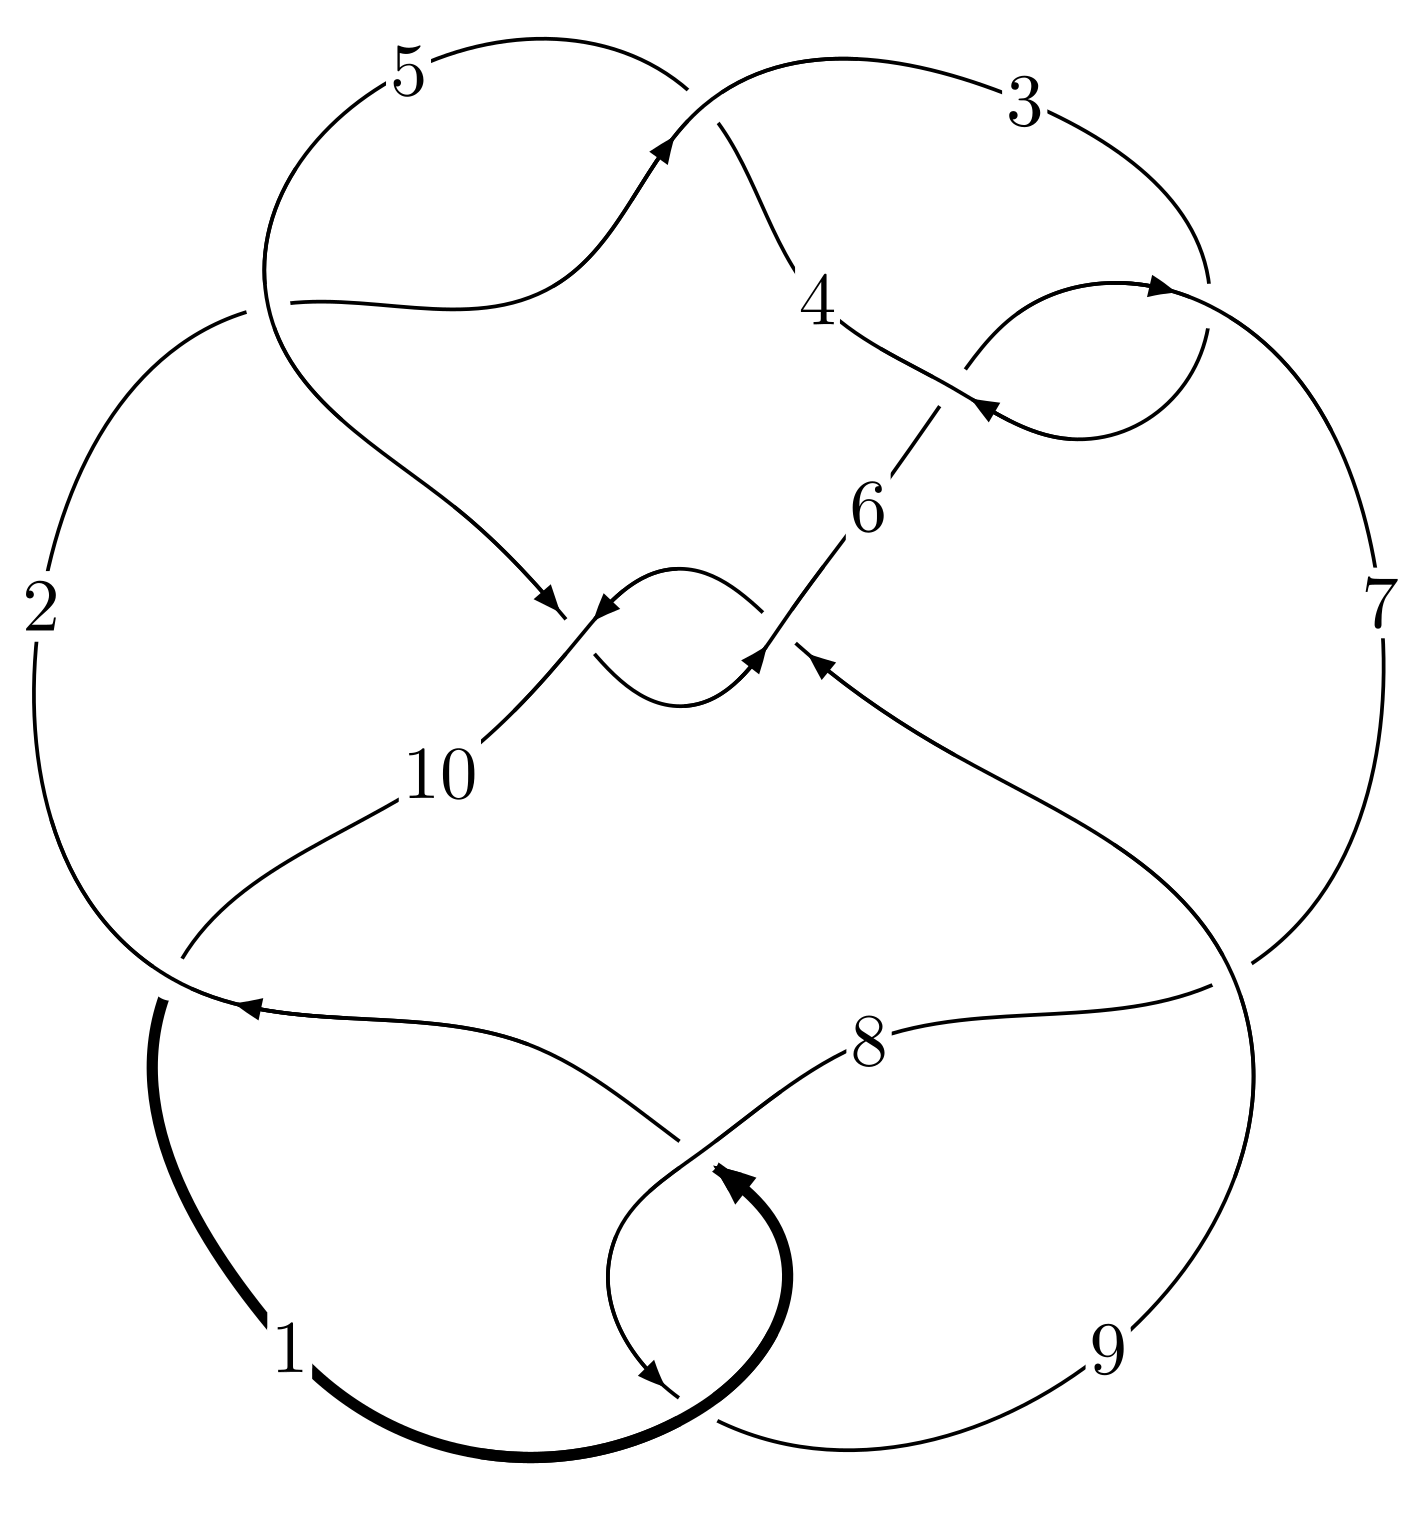
\includegraphics[width=112pt]{../../../GIT/diagram.site/Diagrams/png/142_10_58.png}\\
\ \ \ A knot diagram\footnotemark}&
\allowdisplaybreaks
\textbf{Linearized knot diagam} \\
\cline{2-2}
 &
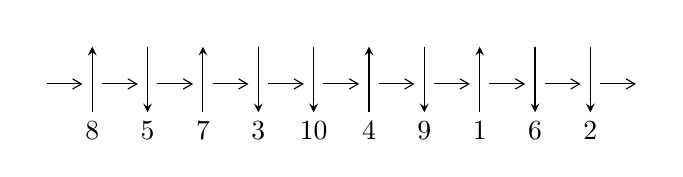
\begin{tikzpicture}[x=20pt, y=17pt]
	% nodes
	\node (C0) at (0, 0) {};
	\node (C1) at (1, 0) {};
	\node (C1U) at (1, +1) {};
	\node (C1D) at (1, -1) {8};

	\node (C2) at (2, 0) {};
	\node (C2U) at (2, +1) {};
	\node (C2D) at (2, -1) {5};

	\node (C3) at (3, 0) {};
	\node (C3U) at (3, +1) {};
	\node (C3D) at (3, -1) {7};

	\node (C4) at (4, 0) {};
	\node (C4U) at (4, +1) {};
	\node (C4D) at (4, -1) {3};

	\node (C5) at (5, 0) {};
	\node (C5U) at (5, +1) {};
	\node (C5D) at (5, -1) {10};

	\node (C6) at (6, 0) {};
	\node (C6U) at (6, +1) {};
	\node (C6D) at (6, -1) {4};

	\node (C7) at (7, 0) {};
	\node (C7U) at (7, +1) {};
	\node (C7D) at (7, -1) {9};

	\node (C8) at (8, 0) {};
	\node (C8U) at (8, +1) {};
	\node (C8D) at (8, -1) {1};

	\node (C9) at (9, 0) {};
	\node (C9U) at (9, +1) {};
	\node (C9D) at (9, -1) {6};

	\node (C10) at (10, 0) {};
	\node (C10U) at (10, +1) {};
	\node (C10D) at (10, -1) {2};
	\node (C11) at (11, 0) {};

	% arrows
	\draw[->,>={angle 60}]
	(C0) edge (C1) (C1) edge (C2) (C2) edge (C3) (C3) edge (C4) (C4) edge (C5) (C5) edge (C6) (C6) edge (C7) (C7) edge (C8) (C8) edge (C9) (C9) edge (C10) (C10) edge (C11) ;	\draw[->,>=stealth]
	(C1D) edge (C1U) (C2U) edge (C2D) (C3D) edge (C3U) (C4U) edge (C4D) (C5U) edge (C5D) (C6D) edge (C6U) (C7U) edge (C7D) (C8D) edge (C8U) (C9U) edge (C9D) (C10U) edge (C10D) ;
	\end{tikzpicture} \\
\hhline{~~} \\& 
\textbf{Solving Sequence} \\ \cline{2-2} 
 &
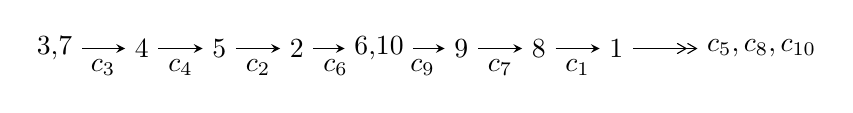
\begin{tikzpicture}[x=28pt, y=7pt]
	% node
	\node (A0) at (-1/8, 0) {3,7};
	\node (A1) at (1, 0) {4};
	\node (A2) at (2, 0) {5};
	\node (A3) at (3, 0) {2};
	\node (A4) at (65/16, 0) {6,10};
	\node (A5) at (41/8, 0) {9};
	\node (A6) at (49/8, 0) {8};
	\node (A7) at (57/8, 0) {1};
	\node (C1) at (1/2, -1) {$c_{3}$};
	\node (C2) at (3/2, -1) {$c_{4}$};
	\node (C3) at (5/2, -1) {$c_{2}$};
	\node (C4) at (7/2, -1) {$c_{6}$};
	\node (C5) at (37/8, -1) {$c_{9}$};
	\node (C6) at (45/8, -1) {$c_{7}$};
	\node (C7) at (53/8, -1) {$c_{1}$};
	\node (A8) at (9, 0) {$c_{5},c_{8},c_{10}$};

	% edge
	\draw[->,>=stealth]	
	(A0) edge (A1) (A1) edge (A2) (A2) edge (A3) (A3) edge (A4) (A4) edge (A5) (A5) edge (A6) (A6) edge (A7) ;
	\draw[->>,>={angle 60}]	
	(A7) edge (A8);
\end{tikzpicture} \\ 

\end{tabular} \\

\footnotetext{
The image of knot diagram is generated by the software ``\textbf{Draw programme}" developed by Andrew Bartholomew(\url{http://www.layer8.co.uk/maths/draw/index.htm\#Running-draw}), where we modified some parts for our purpose(\url{https://github.com/CATsTAILs/LinksPainter}).
}\phantom \\ \newline 
\centering \textbf{Ideals for irreducible components\footnotemark of $X_{\text{par}}$} 
 
\begin{align*}
I^u_{1}&=\langle 
u^7+u^5+2 u^3+b+u,\;- u^6- u^4-2 u^2+a-1,\;u^{10}- u^9+2 u^8- u^7+4 u^6-2 u^5+4 u^4- u^3+3 u^2+u+1\rangle \\
I^u_{2}&=\langle 
u^{25}+2 u^{24}+\cdots+b+3,\;3 u^{25}-7 u^{24}+\cdots+a-6,\;u^{26}-2 u^{25}+\cdots- u+1\rangle \\
I^u_{3}&=\langle 
b+u+1,\;a- u,\;u^2+u+1\rangle \\
I^u_{4}&=\langle 
b- u,\;a-1,\;u^2+u+1\rangle \\
\\
\end{align*}
\raggedright * 4 irreducible components of $\dim_{\mathbb{C}}=0$, with total 40 representations.\\
\footnotetext{All coefficients of polynomials are rational numbers. But the coefficients are sometimes approximated in decimal forms when there is not enough margin.}
\newpage
\renewcommand{\arraystretch}{1}
\centering \section*{I. $I^u_{1}= \langle u^7+u^5+2 u^3+b+u,\;- u^6- u^4-2 u^2+a-1,\;u^{10}- u^9+\cdots+u+1 \rangle$}
\flushleft \textbf{(i) Arc colorings}\\
\begin{tabular}{m{7pt} m{180pt} m{7pt} m{180pt} }
\flushright $a_{3}=$&$\begin{pmatrix}1\\0\end{pmatrix}$ \\
\flushright $a_{7}=$&$\begin{pmatrix}0\\u\end{pmatrix}$ \\
\flushright $a_{4}=$&$\begin{pmatrix}1\\- u^2\end{pmatrix}$ \\
\flushright $a_{5}=$&$\begin{pmatrix}u^2+1\\- u^2\end{pmatrix}$ \\
\flushright $a_{2}=$&$\begin{pmatrix}u^4+u^2+1\\- u^4\end{pmatrix}$ \\
\flushright $a_{6}=$&$\begin{pmatrix}- u\\u^3+u\end{pmatrix}$ \\
\flushright $a_{10}=$&$\begin{pmatrix}u^6+u^4+2 u^2+1\\- u^7- u^5-2 u^3- u\end{pmatrix}$ \\
\flushright $a_{9}=$&$\begin{pmatrix}- u\\u^8- u^7+2 u^6- u^5+3 u^4- u^3+3 u^2+1\end{pmatrix}$ \\
\flushright $a_{8}=$&$\begin{pmatrix}- u^3\\- u^6+u^5- u^4+u^3-2 u^2-1\end{pmatrix}$ \\
\flushright $a_{1}=$&$\begin{pmatrix}u^2+1\\- u^7+u^6- u^5-2 u^3- u\end{pmatrix}$\\&\end{tabular}
\flushleft \textbf{(ii) Obstruction class $= -1$}\\~\\
\flushleft \textbf{(iii) Cusp Shapes $= 4 u^9-6 u^8+6 u^7-4 u^6+14 u^5-14 u^4+10 u^3-6 u^2+10 u$}\\~\\
\newpage\renewcommand{\arraystretch}{1}
\flushleft \textbf{(iv) u-Polynomials at the component}\newline \\
\begin{tabular}{m{50pt}|m{274pt}}
Crossings & \hspace{64pt}u-Polynomials at each crossing \\
\hline $$\begin{aligned}c_{1},c_{3},c_{6}\\c_{8}\end{aligned}$$&$\begin{aligned}
&u^{10}+u^9+2 u^8+u^7+4 u^6+2 u^5+4 u^4+u^3+3 u^2- u+1
\end{aligned}$\\
\hline $$\begin{aligned}c_{2},c_{4},c_{7}\\c_{10}\end{aligned}$$&$\begin{aligned}
&u^{10}+3 u^9+\cdots+5 u+1
\end{aligned}$\\
\hline $$\begin{aligned}c_{5},c_{9}\end{aligned}$$&$\begin{aligned}
&u^{10}-5 u^9+\cdots-8 u+4
\end{aligned}$\\
\hline
\end{tabular}\\~\\
\newpage\renewcommand{\arraystretch}{1}
\flushleft \textbf{(v) Riley Polynomials at the component}\newline \\
\begin{tabular}{m{50pt}|m{274pt}}
Crossings & \hspace{64pt}Riley Polynomials at each crossing \\
\hline $$\begin{aligned}c_{1},c_{3},c_{6}\\c_{8}\end{aligned}$$&$\begin{aligned}
&y^{10}+3 y^9+\cdots+5 y+1
\end{aligned}$\\
\hline $$\begin{aligned}c_{2},c_{4},c_{7}\\c_{10}\end{aligned}$$&$\begin{aligned}
&y^{10}+11 y^9+\cdots+13 y+1
\end{aligned}$\\
\hline $$\begin{aligned}c_{5},c_{9}\end{aligned}$$&$\begin{aligned}
&y^{10}+5 y^9+\cdots+32 y+16
\end{aligned}$\\
\hline
\end{tabular}\\~\\
\newpage\flushleft \textbf{(vi) Complex Volumes and Cusp Shapes}
$$\begin{array}{c|c|c}  
\text{Solutions to }I^u_{1}& \I (\text{vol} + \sqrt{-1}CS) & \text{Cusp shape}\\
 \hline 
\begin{aligned}
u &= -0.100577 + 0.954526 I \\
a &= -0.658857 - 0.498555 I \\
b &= -0.542150 + 0.578753 I\end{aligned}
 & -3.48123 - 2.16643 I & -9.00466 + 4.21901 I \\ \hline\begin{aligned}
u &= -0.100577 - 0.954526 I \\
a &= -0.658857 + 0.498555 I \\
b &= -0.542150 - 0.578753 I\end{aligned}
 & -3.48123 + 2.16643 I & -9.00466 - 4.21901 I \\ \hline\begin{aligned}
u &= \phantom{-}0.900362 + 0.768734 I \\
a &= -1.68093 + 0.92466 I \\
b &= \phantom{-}2.22427 + 0.45966 I\end{aligned}
 & \phantom{-}10.21950 - 0.19532 I & \phantom{-}4.14143 - 1.59060 I \\ \hline\begin{aligned}
u &= \phantom{-}0.900362 - 0.768734 I \\
a &= -1.68093 - 0.92466 I \\
b &= \phantom{-}2.22427 - 0.45966 I\end{aligned}
 & \phantom{-}10.21950 + 0.19532 I & \phantom{-}4.14143 + 1.59060 I \\ \hline\begin{aligned}
u &= -0.774061 + 0.907730 I \\
a &= -0.053403 + 0.383357 I \\
b &= \phantom{-}0.306648 + 0.345217 I\end{aligned}
 & \phantom{-}4.50100 - 5.87397 I & \phantom{-}1.27770 + 5.35715 I \\ \hline\begin{aligned}
u &= -0.774061 - 0.907730 I \\
a &= -0.053403 - 0.383357 I \\
b &= \phantom{-}0.306648 - 0.345217 I\end{aligned}
 & \phantom{-}4.50100 + 5.87397 I & \phantom{-}1.27770 - 5.35715 I \\ \hline\begin{aligned}
u &= \phantom{-}0.782324 + 1.035710 I \\
a &= \phantom{-}1.19625 - 1.47594 I \\
b &= -2.46450 - 0.08430 I\end{aligned}
 & \phantom{-}8.4959 + 12.7213 I & \phantom{-}1.50029 - 7.98966 I \\ \hline\begin{aligned}
u &= \phantom{-}0.782324 - 1.035710 I \\
a &= \phantom{-}1.19625 + 1.47594 I \\
b &= -2.46450 + 0.08430 I\end{aligned}
 & \phantom{-}8.4959 - 12.7213 I & \phantom{-}1.50029 + 7.98966 I \\ \hline\begin{aligned}
u &= -0.308049 + 0.477623 I \\
a &= \phantom{-}0.696944 - 0.500305 I \\
b &= -0.024265 - 0.486995 I\end{aligned}
 & \phantom{-}0.004061 - 1.246020 I & \phantom{-}0.08524 + 5.02615 I \\ \hline\begin{aligned}
u &= -0.308049 - 0.477623 I \\
a &= \phantom{-}0.696944 + 0.500305 I \\
b &= -0.024265 + 0.486995 I\end{aligned}
 & \phantom{-}0.004061 + 1.246020 I & \phantom{-}0.08524 - 5.02615 I\\
 \hline 
 \end{array}$$\newpage\newpage\renewcommand{\arraystretch}{1}
\centering \section*{II. $I^u_{2}= \langle u^{25}+2 u^{24}+\cdots+b+3,\;3 u^{25}-7 u^{24}+\cdots+a-6,\;u^{26}-2 u^{25}+\cdots- u+1 \rangle$}
\flushleft \textbf{(i) Arc colorings}\\
\begin{tabular}{m{7pt} m{180pt} m{7pt} m{180pt} }
\flushright $a_{3}=$&$\begin{pmatrix}1\\0\end{pmatrix}$ \\
\flushright $a_{7}=$&$\begin{pmatrix}0\\u\end{pmatrix}$ \\
\flushright $a_{4}=$&$\begin{pmatrix}1\\- u^2\end{pmatrix}$ \\
\flushright $a_{5}=$&$\begin{pmatrix}u^2+1\\- u^2\end{pmatrix}$ \\
\flushright $a_{2}=$&$\begin{pmatrix}u^4+u^2+1\\- u^4\end{pmatrix}$ \\
\flushright $a_{6}=$&$\begin{pmatrix}- u\\u^3+u\end{pmatrix}$ \\
\flushright $a_{10}=$&$\begin{pmatrix}-3 u^{25}+7 u^{24}+\cdots-4 u+6\\- u^{25}-2 u^{24}+\cdots-3 u-3\end{pmatrix}$ \\
\flushright $a_{9}=$&$\begin{pmatrix}- u^{25}+3 u^{24}+\cdots-2 u+4\\- u^{22}-3 u^{20}+\cdots-3 u-1\end{pmatrix}$ \\
\flushright $a_{8}=$&$\begin{pmatrix}- u^{25}+u^{24}+\cdots-3 u-1\\u^{25}-2 u^{24}+\cdots+3 u-1\end{pmatrix}$ \\
\flushright $a_{1}=$&$\begin{pmatrix}- u^{25}+3 u^{24}+\cdots- u+5\\- u^{25}-4 u^{23}+\cdots-3 u-2\end{pmatrix}$\\&\end{tabular}
\flushleft \textbf{(ii) Obstruction class $= -1$}\\~\\
\flushleft \textbf{(iii) Cusp Shapes $= 5 u^{25}-12 u^{24}+25 u^{23}-43 u^{22}+75 u^{21}-109 u^{20}+126 u^{19}-175 u^{18}+168 u^{17}-200 u^{16}+98 u^{15}-164 u^{14}-6 u^{13}-49 u^{12}-144 u^{11}-10 u^{10}-179 u^9+26 u^8-112 u^7-28 u^6-47 u^5-26 u^4+9 u^3-16 u^2+15 u-5$}\\~\\
\newpage\renewcommand{\arraystretch}{1}
\flushleft \textbf{(iv) u-Polynomials at the component}\newline \\
\begin{tabular}{m{50pt}|m{274pt}}
Crossings & \hspace{64pt}u-Polynomials at each crossing \\
\hline $$\begin{aligned}c_{1},c_{3},c_{6}\\c_{8}\end{aligned}$$&$\begin{aligned}
&u^{26}+2 u^{25}+\cdots+u+1
\end{aligned}$\\
\hline $$\begin{aligned}c_{2},c_{4},c_{7}\\c_{10}\end{aligned}$$&$\begin{aligned}
&u^{26}+8 u^{25}+\cdots+13 u+1
\end{aligned}$\\
\hline $$\begin{aligned}c_{5},c_{9}\end{aligned}$$&$\begin{aligned}
&(u^{13}+2 u^{12}+\cdots+3 u+2)^{2}
\end{aligned}$\\
\hline
\end{tabular}\\~\\
\newpage\renewcommand{\arraystretch}{1}
\flushleft \textbf{(v) Riley Polynomials at the component}\newline \\
\begin{tabular}{m{50pt}|m{274pt}}
Crossings & \hspace{64pt}Riley Polynomials at each crossing \\
\hline $$\begin{aligned}c_{1},c_{3},c_{6}\\c_{8}\end{aligned}$$&$\begin{aligned}
&y^{26}+8 y^{25}+\cdots+13 y+1
\end{aligned}$\\
\hline $$\begin{aligned}c_{2},c_{4},c_{7}\\c_{10}\end{aligned}$$&$\begin{aligned}
&y^{26}+20 y^{25}+\cdots-11 y+1
\end{aligned}$\\
\hline $$\begin{aligned}c_{5},c_{9}\end{aligned}$$&$\begin{aligned}
&(y^{13}+10 y^{12}+\cdots-7 y-4)^{2}
\end{aligned}$\\
\hline
\end{tabular}\\~\\
\newpage\flushleft \textbf{(vi) Complex Volumes and Cusp Shapes}
$$\begin{array}{c|c|c}  
\text{Solutions to }I^u_{2}& \I (\text{vol} + \sqrt{-1}CS) & \text{Cusp shape}\\
 \hline 
\begin{aligned}
u &= \phantom{-}0.752045 + 0.803934 I \\
a &= \phantom{-}1.97258 - 1.23710 I \\
b &= -2.47801 - 0.65547 I\end{aligned}
 & \phantom{-}1.88524 - 0.96841 I & \phantom{-}0.413632 + 1.140295 I \\ \hline\begin{aligned}
u &= \phantom{-}0.752045 - 0.803934 I \\
a &= \phantom{-}1.97258 + 1.23710 I \\
b &= -2.47801 + 0.65547 I\end{aligned}
 & \phantom{-}1.88524 + 0.96841 I & \phantom{-}0.413632 - 1.140295 I \\ \hline\begin{aligned}
u &= -0.578645 + 0.950081 I \\
a &= \phantom{-}0.030039 + 0.285319 I \\
b &= \phantom{-}0.288458 + 0.136559 I\end{aligned}
 & -0.80957 - 3.02973 I & -5.16840 + 1.62282 I \\ \hline\begin{aligned}
u &= -0.578645 - 0.950081 I \\
a &= \phantom{-}0.030039 - 0.285319 I \\
b &= \phantom{-}0.288458 - 0.136559 I\end{aligned}
 & -0.80957 + 3.02973 I & -5.16840 - 1.62282 I \\ \hline\begin{aligned}
u &= -0.496478 + 0.720203 I \\
a &= \phantom{-}0.299461 - 0.224790 I \\
b &= -0.013218 - 0.327276 I\end{aligned}
 & \phantom{-}0.00150 - 1.41503 I & -1.90513 + 4.60201 I \\ \hline\begin{aligned}
u &= -0.496478 - 0.720203 I \\
a &= \phantom{-}0.299461 + 0.224790 I \\
b &= -0.013218 + 0.327276 I\end{aligned}
 & \phantom{-}0.00150 + 1.41503 I & -1.90513 - 4.60201 I \\ \hline\begin{aligned}
u &= -0.335785 + 1.109920 I \\
a &= \phantom{-}0.267955 + 0.444237 I \\
b &= \phantom{-}0.583042 - 0.148240 I\end{aligned}
 & \phantom{-}1.88524 - 0.96841 I & \phantom{-}0.413632 + 1.140295 I \\ \hline\begin{aligned}
u &= -0.335785 - 1.109920 I \\
a &= \phantom{-}0.267955 - 0.444237 I \\
b &= \phantom{-}0.583042 + 0.148240 I\end{aligned}
 & \phantom{-}1.88524 + 0.96841 I & \phantom{-}0.413632 - 1.140295 I \\ \hline\begin{aligned}
u &= \phantom{-}0.905446 + 0.730041 I \\
a &= \phantom{-}1.71372 - 0.85399 I \\
b &= -2.17513 - 0.47784 I\end{aligned}
 & \phantom{-}9.45063 - 6.48172 I & \phantom{-}3.04187 + 3.27257 I \\ \hline\begin{aligned}
u &= \phantom{-}0.905446 - 0.730041 I \\
a &= \phantom{-}1.71372 + 0.85399 I \\
b &= -2.17513 + 0.47784 I\end{aligned}
 & \phantom{-}9.45063 + 6.48172 I & \phantom{-}3.04187 - 3.27257 I\\
 \hline 
 \end{array}$$\newpage$$\begin{array}{c|c|c}  
\text{Solutions to }I^u_{2}& \I (\text{vol} + \sqrt{-1}CS) & \text{Cusp shape}\\
 \hline 
\begin{aligned}
u &= -0.269616 + 1.131670 I \\
a &= -0.308288 - 0.503667 I \\
b &= -0.653102 + 0.213082 I\end{aligned}
 & \phantom{-}1.46125 - 6.61332 I & -1.15142 + 6.72912 I \\ \hline\begin{aligned}
u &= -0.269616 - 1.131670 I \\
a &= -0.308288 + 0.503667 I \\
b &= -0.653102 - 0.213082 I\end{aligned}
 & \phantom{-}1.46125 + 6.61332 I & -1.15142 - 6.72912 I \\ \hline\begin{aligned}
u &= -0.786233 + 0.860060 I \\
a &= \phantom{-}0.072545 - 0.387289 I \\
b &= -0.276054 - 0.366893 I\end{aligned}
 & \phantom{-}4.64840\phantom{ +0.000000I} & \phantom{-}1.75564 + 0. I\phantom{ +0.000000I} \\ \hline\begin{aligned}
u &= -0.786233 - 0.860060 I \\
a &= \phantom{-}0.072545 + 0.387289 I \\
b &= -0.276054 + 0.366893 I\end{aligned}
 & \phantom{-}4.64840\phantom{ +0.000000I} & \phantom{-}1.75564 + 0. I\phantom{ +0.000000I} \\ \hline\begin{aligned}
u &= -0.819468 + 0.042718 I \\
a &= \phantom{-}0.021039 - 0.644673 I \\
b &= -0.010298 - 0.529188 I\end{aligned}
 & \phantom{-}5.42596 - 2.97283 I & \phantom{-}4.39163 + 2.88376 I \\ \hline\begin{aligned}
u &= -0.819468 - 0.042718 I \\
a &= \phantom{-}0.021039 + 0.644673 I \\
b &= -0.010298 + 0.529188 I\end{aligned}
 & \phantom{-}5.42596 + 2.97283 I & \phantom{-}4.39163 - 2.88376 I \\ \hline\begin{aligned}
u &= \phantom{-}0.791857 + 0.886903 I \\
a &= -1.65384 + 1.34745 I \\
b &= \phantom{-}2.50466 + 0.39980 I\end{aligned}
 & \phantom{-}5.42596 + 2.97283 I & \phantom{-}4.39163 - 2.88376 I \\ \hline\begin{aligned}
u &= \phantom{-}0.791857 - 0.886903 I \\
a &= -1.65384 - 1.34745 I \\
b &= \phantom{-}2.50466 - 0.39980 I\end{aligned}
 & \phantom{-}5.42596 - 2.97283 I & \phantom{-}4.39163 + 2.88376 I \\ \hline\begin{aligned}
u &= \phantom{-}0.732196 + 0.941652 I \\
a &= \phantom{-}1.54369 - 1.64448 I \\
b &= -2.67881 - 0.24953 I\end{aligned}
 & \phantom{-}1.46125 + 6.61332 I & -1.15142 - 6.72912 I \\ \hline\begin{aligned}
u &= \phantom{-}0.732196 - 0.941652 I \\
a &= \phantom{-}1.54369 + 1.64448 I \\
b &= -2.67881 + 0.24953 I\end{aligned}
 & \phantom{-}1.46125 - 6.61332 I & -1.15142 + 6.72912 I\\
 \hline 
 \end{array}$$\newpage$$\begin{array}{c|c|c}  
\text{Solutions to }I^u_{2}& \I (\text{vol} + \sqrt{-1}CS) & \text{Cusp shape}\\
 \hline 
\begin{aligned}
u &= \phantom{-}0.156803 + 0.747604 I \\
a &= -1.50536 - 0.52470 I \\
b &= -0.156223 + 1.207680 I\end{aligned}
 & -0.80957 + 3.02973 I & -5.16840 - 1.62282 I \\ \hline\begin{aligned}
u &= \phantom{-}0.156803 - 0.747604 I \\
a &= -1.50536 + 0.52470 I \\
b &= -0.156223 - 1.207680 I\end{aligned}
 & -0.80957 - 3.02973 I & -5.16840 + 1.62282 I \\ \hline\begin{aligned}
u &= \phantom{-}0.799863 + 1.014160 I \\
a &= -1.26195 + 1.42943 I \\
b &= \phantom{-}2.45906 + 0.13647 I\end{aligned}
 & \phantom{-}9.45063 + 6.48172 I & \phantom{-}3.04187 - 3.27257 I \\ \hline\begin{aligned}
u &= \phantom{-}0.799863 - 1.014160 I \\
a &= -1.26195 - 1.42943 I \\
b &= \phantom{-}2.45906 - 0.13647 I\end{aligned}
 & \phantom{-}9.45063 - 6.48172 I & \phantom{-}3.04187 + 3.27257 I \\ \hline\begin{aligned}
u &= \phantom{-}0.148015 + 0.419312 I \\
a &= \phantom{-}1.80840 - 0.30217 I \\
b &= -0.394374 - 0.713561 I\end{aligned}
 & \phantom{-}0.00150 - 1.41503 I & -1.90513 + 4.60201 I \\ \hline\begin{aligned}
u &= \phantom{-}0.148015 - 0.419312 I \\
a &= \phantom{-}1.80840 + 0.30217 I \\
b &= -0.394374 + 0.713561 I\end{aligned}
 & \phantom{-}0.00150 + 1.41503 I & -1.90513 - 4.60201 I\\
 \hline 
 \end{array}$$\newpage\newpage\renewcommand{\arraystretch}{1}
\centering \section*{III. $I^u_{3}= \langle b+u+1,\;a- u,\;u^2+u+1 \rangle$}
\flushleft \textbf{(i) Arc colorings}\\
\begin{tabular}{m{7pt} m{180pt} m{7pt} m{180pt} }
\flushright $a_{3}=$&$\begin{pmatrix}1\\0\end{pmatrix}$ \\
\flushright $a_{7}=$&$\begin{pmatrix}0\\u\end{pmatrix}$ \\
\flushright $a_{4}=$&$\begin{pmatrix}1\\u+1\end{pmatrix}$ \\
\flushright $a_{5}=$&$\begin{pmatrix}- u\\u+1\end{pmatrix}$ \\
\flushright $a_{2}=$&$\begin{pmatrix}0\\- u\end{pmatrix}$ \\
\flushright $a_{6}=$&$\begin{pmatrix}- u\\u+1\end{pmatrix}$ \\
\flushright $a_{10}=$&$\begin{pmatrix}u\\- u-1\end{pmatrix}$ \\
\flushright $a_{9}=$&$\begin{pmatrix}u\\- u-1\end{pmatrix}$ \\
\flushright $a_{8}=$&$\begin{pmatrix}-1\\0\end{pmatrix}$ \\
\flushright $a_{1}=$&$\begin{pmatrix}u\\- u\end{pmatrix}$\\&\end{tabular}
\flushleft \textbf{(ii) Obstruction class $= 1$}\\~\\
\flushleft \textbf{(iii) Cusp Shapes $= 8 u+4$}\\~\\
\newpage\renewcommand{\arraystretch}{1}
\flushleft \textbf{(iv) u-Polynomials at the component}\newline \\
\begin{tabular}{m{50pt}|m{274pt}}
Crossings & \hspace{64pt}u-Polynomials at each crossing \\
\hline $$\begin{aligned}c_{1},c_{2},c_{6}\\c_{7},c_{10}\end{aligned}$$&$\begin{aligned}
&u^2- u+1
\end{aligned}$\\
\hline $$\begin{aligned}c_{3},c_{4},c_{8}\end{aligned}$$&$\begin{aligned}
&u^2+u+1
\end{aligned}$\\
\hline $$\begin{aligned}c_{5},c_{9}\end{aligned}$$&$\begin{aligned}
&u^2
\end{aligned}$\\
\hline
\end{tabular}\\~\\
\newpage\renewcommand{\arraystretch}{1}
\flushleft \textbf{(v) Riley Polynomials at the component}\newline \\
\begin{tabular}{m{50pt}|m{274pt}}
Crossings & \hspace{64pt}Riley Polynomials at each crossing \\
\hline $$\begin{aligned}c_{1},c_{2},c_{3}\\c_{4},c_{6},c_{7}\\c_{8},c_{10}\end{aligned}$$&$\begin{aligned}
&y^2+y+1
\end{aligned}$\\
\hline $$\begin{aligned}c_{5},c_{9}\end{aligned}$$&$\begin{aligned}
&y^2
\end{aligned}$\\
\hline
\end{tabular}\\~\\
\newpage\flushleft \textbf{(vi) Complex Volumes and Cusp Shapes}
$$\begin{array}{c|c|c}  
\text{Solutions to }I^u_{3}& \I (\text{vol} + \sqrt{-1}CS) & \text{Cusp shape}\\
 \hline 
\begin{aligned}
u &= -0.500000 + 0.866025 I \\
a &= -0.500000 + 0.866025 I \\
b &= -0.500000 - 0.866025 I\end{aligned}
 & \phantom{-0.000000 } -4.05977 I & \phantom{-0.000000 -}0. + 6.92820 I \\ \hline\begin{aligned}
u &= -0.500000 - 0.866025 I \\
a &= -0.500000 - 0.866025 I \\
b &= -0.500000 + 0.866025 I\end{aligned}
 & \phantom{-0.000000 -}4.05977 I & \phantom{-0.000000 } 0. - 6.92820 I\\
 \hline 
 \end{array}$$\newpage\newpage\renewcommand{\arraystretch}{1}
\centering \section*{IV. $I^u_{4}= \langle b- u,\;a-1,\;u^2+u+1 \rangle$}
\flushleft \textbf{(i) Arc colorings}\\
\begin{tabular}{m{7pt} m{180pt} m{7pt} m{180pt} }
\flushright $a_{3}=$&$\begin{pmatrix}1\\0\end{pmatrix}$ \\
\flushright $a_{7}=$&$\begin{pmatrix}0\\u\end{pmatrix}$ \\
\flushright $a_{4}=$&$\begin{pmatrix}1\\u+1\end{pmatrix}$ \\
\flushright $a_{5}=$&$\begin{pmatrix}- u\\u+1\end{pmatrix}$ \\
\flushright $a_{2}=$&$\begin{pmatrix}0\\- u\end{pmatrix}$ \\
\flushright $a_{6}=$&$\begin{pmatrix}- u\\u+1\end{pmatrix}$ \\
\flushright $a_{10}=$&$\begin{pmatrix}1\\u\end{pmatrix}$ \\
\flushright $a_{9}=$&$\begin{pmatrix}1\\u\end{pmatrix}$ \\
\flushright $a_{8}=$&$\begin{pmatrix}- u\\2 u+1\end{pmatrix}$ \\
\flushright $a_{1}=$&$\begin{pmatrix}1\\-1\end{pmatrix}$\\&\end{tabular}
\flushleft \textbf{(ii) Obstruction class $= 1$}\\~\\
\flushleft \textbf{(iii) Cusp Shapes $= -3$}\\~\\
\newpage\renewcommand{\arraystretch}{1}
\flushleft \textbf{(iv) u-Polynomials at the component}\newline \\
\begin{tabular}{m{50pt}|m{274pt}}
Crossings & \hspace{64pt}u-Polynomials at each crossing \\
\hline $$\begin{aligned}c_{1},c_{2},c_{6}\\c_{7},c_{10}\end{aligned}$$&$\begin{aligned}
&u^2- u+1
\end{aligned}$\\
\hline $$\begin{aligned}c_{3},c_{4},c_{8}\end{aligned}$$&$\begin{aligned}
&u^2+u+1
\end{aligned}$\\
\hline $$\begin{aligned}c_{5},c_{9}\end{aligned}$$&$\begin{aligned}
&u^2
\end{aligned}$\\
\hline
\end{tabular}\\~\\
\newpage\renewcommand{\arraystretch}{1}
\flushleft \textbf{(v) Riley Polynomials at the component}\newline \\
\begin{tabular}{m{50pt}|m{274pt}}
Crossings & \hspace{64pt}Riley Polynomials at each crossing \\
\hline $$\begin{aligned}c_{1},c_{2},c_{3}\\c_{4},c_{6},c_{7}\\c_{8},c_{10}\end{aligned}$$&$\begin{aligned}
&y^2+y+1
\end{aligned}$\\
\hline $$\begin{aligned}c_{5},c_{9}\end{aligned}$$&$\begin{aligned}
&y^2
\end{aligned}$\\
\hline
\end{tabular}\\~\\
\newpage\flushleft \textbf{(vi) Complex Volumes and Cusp Shapes}
$$\begin{array}{c|c|c}  
\text{Solutions to }I^u_{4}& \I (\text{vol} + \sqrt{-1}CS) & \text{Cusp shape}\\
 \hline 
\begin{aligned}
u &= -0.500000 + 0.866025 I \\
a &= \phantom{-}1.00000\phantom{ +0.000000I} \\
b &= -0.500000 + 0.866025 I\end{aligned}
 & \phantom{-0.000000 } 0 & -3.00000\phantom{ +0.000000I} \\ \hline\begin{aligned}
u &= -0.500000 - 0.866025 I \\
a &= \phantom{-}1.00000\phantom{ +0.000000I} \\
b &= -0.500000 - 0.866025 I\end{aligned}
 & \phantom{-0.000000 } 0 & -3.00000\phantom{ +0.000000I}\\
 \hline 
 \end{array}$$\newpage
\newpage\renewcommand{\arraystretch}{1}
\centering \section*{ V. u-Polynomials}
\begin{tabular}{m{50pt}|m{274pt}}
Crossings & \hspace{64pt}u-Polynomials at each crossing \\
\hline $$\begin{aligned}c_{1},c_{6}\end{aligned}$$&$\begin{aligned}
&((u^2- u+1)^2)(u^{10}+u^9+\cdots- u+1)\\
&\cdot(u^{26}+2 u^{25}+\cdots+u+1)
\end{aligned}$\\
\hline $$\begin{aligned}c_{2},c_{7},c_{10}\end{aligned}$$&$\begin{aligned}
&((u^2- u+1)^2)(u^{10}+3 u^9+\cdots+5 u+1)(u^{26}+8 u^{25}+\cdots+13 u+1)
\end{aligned}$\\
\hline $$\begin{aligned}c_{3},c_{8}\end{aligned}$$&$\begin{aligned}
&((u^2+u+1)^2)(u^{10}+u^9+\cdots- u+1)\\
&\cdot(u^{26}+2 u^{25}+\cdots+u+1)
\end{aligned}$\\
\hline $$\begin{aligned}c_{4}\end{aligned}$$&$\begin{aligned}
&((u^2+u+1)^2)(u^{10}+3 u^9+\cdots+5 u+1)(u^{26}+8 u^{25}+\cdots+13 u+1)
\end{aligned}$\\
\hline $$\begin{aligned}c_{5},c_{9}\end{aligned}$$&$\begin{aligned}
&u^4(u^{10}-5 u^9+\cdots-8 u+4)(u^{13}+2 u^{12}+\cdots+3 u+2)^{2}
\end{aligned}$\\
\hline
\end{tabular}\newpage\renewcommand{\arraystretch}{1}
\centering \section*{ VI. Riley Polynomials}
\begin{tabular}{m{50pt}|m{274pt}}
Crossings & \hspace{64pt}Riley Polynomials at each crossing \\
\hline $$\begin{aligned}c_{1},c_{3},c_{6}\\c_{8}\end{aligned}$$&$\begin{aligned}
&((y^2+y+1)^2)(y^{10}+3 y^9+\cdots+5 y+1)(y^{26}+8 y^{25}+\cdots+13 y+1)
\end{aligned}$\\
\hline $$\begin{aligned}c_{2},c_{4},c_{7}\\c_{10}\end{aligned}$$&$\begin{aligned}
&((y^2+y+1)^2)(y^{10}+11 y^9+\cdots+13 y+1)(y^{26}+20 y^{25}+\cdots-11 y+1)
\end{aligned}$\\
\hline $$\begin{aligned}c_{5},c_{9}\end{aligned}$$&$\begin{aligned}
&y^4(y^{10}+5 y^9+\cdots+32 y+16)(y^{13}+10 y^{12}+\cdots-7 y-4)^{2}
\end{aligned}$\\
\hline
\end{tabular}
\vskip 2pc
\end{document}